\subsection{The S+P Transform}

\subsubsection{Motivation and High-Level Overview}

To address the need for invertibility without inflating the dynamic range in the process of compression, the S+P transform (Sequential transform + Prediction), originally proposed by Said and Pearlman~\cite{said1993sp}, employs a simple combination of a Haar-like multiresolution transform (the ``S'' stage) and an embedded predictive coding stage (the ``P'' stage).

In the broader context of our project, we treat S+P as a hybrid transform that lives between classical wavelet/subband decompositions(transform) and purely predictive schemes. Earlier sections introduce transform coding and the Haar wavelet; here, we focus on what S+P adds on top of that baseline, and how those additions behave inside our JPEG-style pipeline.

Operationally, S+P still proceeds along one-dimensional signals (rows or columns of an image). The S stage performs an integer lifting-style average/difference, producing lowpass (approximate local averages) and highpass (local differences). The P stage then applies an \emph{integer} prediction filter directly to the highpass branch, aiming to decorrelate it further before quantization and entropy coding. Recursively applying S+P to the lowpass component yields the same LL/HL/LH/HH multiresolution layout as Haar, but with much stronger whitening in the highpass bands and stricter control over rounding and borders.

\subsubsection{Sequential Transform (S) Recap}

We briefly recall the 1D S stage, which is the integer analogue of the Haar lifting step. Let $c[n]$ be a sequence of integer samples of length $N$. For each pair $(c[2n], c[2n+1])$ we define
\begin{align}
    d_1[n] &= c[2n+1] - c[2n], \\
    s[n]   &= c[2n] + \left\lfloor \frac{d_1[n]}{2} \right\rfloor,
\end{align}
for $n = 0, \dots, \lfloor N/2 \rfloor - 1$. Here $s[n]$ acts as a local average, while $d_1[n]$ stores the corresponding difference as detail.

This mapping is exactly reversible with integer arithmetic:
\begin{align}
    c[2n]   &= s[n] - \left\lfloor \frac{d_1[n]}{2} \right\rfloor, \\
    c[2n+1] &= c[2n] + d_1[n].
\end{align}
No fractional bits are introduced: only additions, subtractions, and integer floor-divisions by powers of two are used. Applying this S step to all rows and then all columns, and recursing only on the LL quadrant, gives the same multilevel LL/HL/LH/HH pyramid described for the Haar transform, but now entirely in integers. As shown in Figure ~\ref{fig:sp_level1}, each level of S+P transform decompose the image into the four subbands: LL carries the coarse approximation as the mean image of the original, HL captures vertical edges, LH captures horizontal edges, and HH captures fine diagonal texture (the highpass details are scaled up to be more visible). After the second level of decomposition, the LL band can be transformed again to give a multiresolution pyramid, as shown in Figure \ref{fig:sp_level2}. The recursion would continue until one dimension cannot be halved.

\begin{figure}[ht]
    \centering
    \begin{tikzpicture}
        \node[inner sep=0] (img)
            {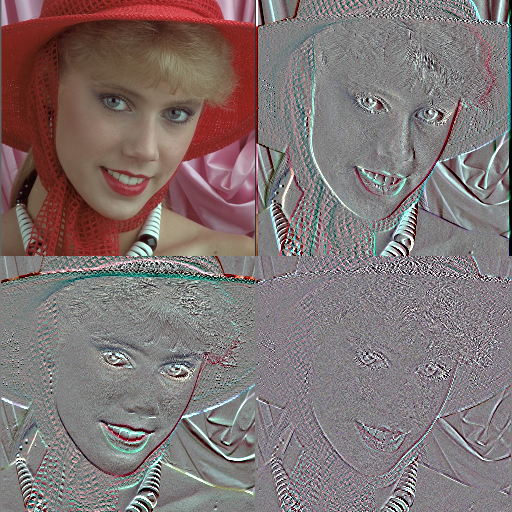
\includegraphics[width=0.90\linewidth]{methods/figures/SP_Level1.png}};

        % labels in each corner
        \node[anchor=north west, font=\medium\bfseries,
              xshift=-18pt, yshift=-4pt] at (img.north west) {LL};
        \node[anchor=north east, font=\medium\bfseries,
              xshift=18pt, yshift=-4pt] at (img.north east) {HL};
        \node[anchor=south west, font=\medium\bfseries,
              xshift=-18pt, yshift=4pt] at (img.south west) {LH};
        \node[anchor{south east}, font=\medium\bfseries,
              xshift=12pt, yshift=6pt] at (img.south east) {HH};
    \end{tikzpicture}
    \caption{One level of the S+P transform.}
    \label{fig:sp_level1}
\end{figure}

\begin{figure}[ht]
    \centering
    \begin{tikzpicture}
        \node[inner sep=0] (img)
            {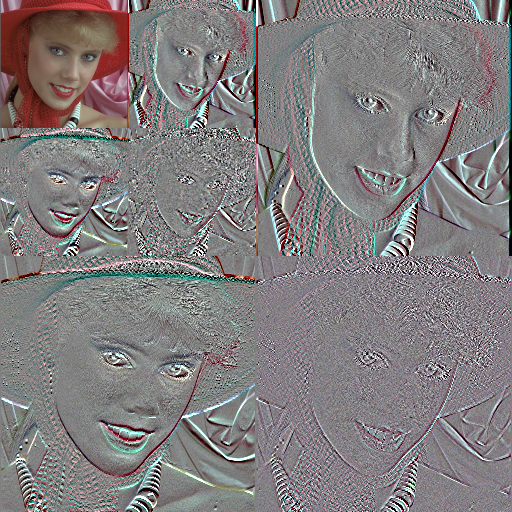
\includegraphics[width=0.90\linewidth]{methods/figures/SP_Level2.png}};

        % labels in each corner
        \node[anchor=north west, font=\medium\bfseries,
              xshift=-22pt, yshift=-4pt] at (img.north west) {LL2};
        \node[anchor=north west, font=\medium\bfseries,
              xshift=-22pt, yshift=8pt] at (img.west) {LH2};
        \node[anchor=north west, font=\medium\bfseries,
              xshift=-22pt, yshift=12pt] at (img.north) {HL2};
        \node[anchor=north west, font=\medium\bfseries,
              xshift=-22pt, yshift=8pt] at (img.center) {HH2};
        \node[anchor=north east, font=\medium\bfseries,
        \node[anchor=north east, font=\medium\bfseries,
              xshift=22pt, yshift=-4pt] at (img.north east) {HL1};
        \node[anchor=south west, font=\medium\bfseries,
              xshift=-22pt, yshift=4pt] at (img.south west) {LH1};
        \node[anchor{south east}, font=\medium\bfseries,
              xshift=12pt, yshift=6pt] at (img.south east) {HH1};
    \end{tikzpicture}
    \caption{Two levels of the S+P transform.}
    \label{fig:sp_level2}
\end{figure}

The correlation coefficient measures the normalized linear dependence between two adjacent data points, ranging from −1 to 1, with higher positive values indicating stronger similarity. Under mild correlation assumptions—in particular, when adjacent samples have correlation coefficient larger than $\tfrac{1}{3}$—S alone already reduces the average variance of the low- and highpass components relative to the original signal~\cite{said1993sp}. The P stage is specifically designed to exploit the residual correlation that remains, mainly in the highpass bands.

\subsubsection{The S+P Transform: Prediction Embedded in the Transform}

The S+P transform augments the S stage with a predictive step that operates directly on the highpass coefficients produced at each one-dimensional pass. Conceptually, we distinguish three sequences:
\begin{itemize}
    \item $s[n]$: the lowpass component after the S stage,
    \item $d_1[n]$: the intermediate highpass component (exact differences),
    \item $d[n]$: the final highpass residual after prediction.
\end{itemize}

\subsubsection{Predictor structure}

We introduce a simple notation for local lowpass differences:
\begin{equation}
    z_\ell[n] = s[n-1] - s[n],
\end{equation}
where $ \ell$ captures local gradients in the lowpass band. Following~\cite{said1993sp}, we estimate $d_1[n]$ from neighboring lowpass samples and the next highpass value $d_1[n+1]$. A generic linear estimator has the form
\begin{equation}
\begin{aligned}
\hat d_1[n] 
    &= \beta_{-1} \, z_\ell[n] 
     + \beta_0   \, z_\ell[n+1] \\
    &\quad + \beta_{+1} \, z_\ell[n+2]
     - \phi_1 \, d_1[n+1].
\end{aligned}
\end{equation}

where $\beta_{-1}, \beta_0, \beta_{+1}, \phi_1$ are predictor coefficients. Intuitively, the first three terms exploit smoothness in the lowpass band, while the last term models correlation between adjacent highpass coefficients. These coefficients were originally obtained by fitting a local linear model to natural and medical images so as to 
minimize the mean–square prediction error of $d_1[n]$ given neighboring lowpass differences and the next highpass 
sample. The fitted values for $(\beta_{-1},\beta_0,\beta_{+1},\phi_1)$ are fixed and do not depend on the image, 
allowing the transform to remain perfectly reversible prior to quantization. For our implementation we use the coefficient set
\[
\beta_{-1}=-1,\qquad \beta_0=2,\qquad \beta_{+1}=-1,\qquad \phi_1=1,
\]
which is the recommended configuration from~\cite{said1993sp}.


To preserve integer reversibility, we do not subtract $\hat{d}_1[n]$ directly. Instead, we perform a quantized correction using an integer denominator $K = 2^{k}$:
\begin{equation}
    \mathrm{pred}[n] = \left\lfloor \frac{\hat{d}_1[n]}{K} \right\rfloor,
\end{equation}
and define the residual
\begin{equation}
    d[n] = d_1[n] - \mathrm{pred}[n].
\end{equation}
The final transformed highpass component is thus $d[n]$, and $d_1[n]$ never needs to be stored explicitly beyond the prediction step.

\subsubsection{Inverse S+P and exact reconstruction}

The inverse transform proceeds in the reverse order of the forward transform. During the inverse of a one-dimensional pass, we assume that $s[n]$ and $d[n]$ are available. We reconstruct $d_1[n]$ by reapplying the same predictor in reverse:
\begin{enumerate}
    \item Visit indices in descending order $n = N/2-1, \dots, 0$, ensuring that $d_1[n+1]$ is already reconstructed when needed.
    \item For each $n$, compute the same predictor numerator using current $s[\cdot]$ and $d_1[n+1]$.
    \item Recompute $\mathrm{pred}[n] = \left\lfloor \hat{d}_1[n] / K \right\rfloor$ and add it back:
    \begin{equation}
        d_1[n] = d[n] + \mathrm{pred}[n].
    \end{equation}
\end{enumerate}
Once $d_1[n]$ is recovered for all $n$, the inverse S transform recovers the original samples $c[2n]$ and $c[2n+1]$ exactly. The crucial point is that the predictor and its quantization are perfectly reproducible during inversion, so no information is lost.

% In our implementation, we adopt a parameterization closely aligned with the ``natural image'' predictor family in~\cite{said1993sp}, but we expose $\beta_{-1}$, $\beta_0$, $\beta_{+1}$, $\phi_1$, and the shift $k$ as tunable parameters. This makes it possible to experiment with both conservative predictors (small attenuation, robust on textured images) and more aggressive ones (strong low-frequency attenuation, favorable on smooth images).
\subsubsection{Frequency-Domain Interpretation}

Although the S+P transform is defined via local integer operations, its behavior is illuminating when viewed in the frequency domain. If we ignore truncation for the sake of analysis and treat the operations as linear, the mapping from the original sequence $c[n]$ to the highpass residual $d[n]$ can be represented as a linear time-invariant filter with a frequency response $F(\mathrm{e}^{j\omega})$.

The S stage alone already suppresses low frequencies in the highpass band, but it does so relatively mildly; the resulting highpass spectrum still exhibits considerable low-frequency energy due to the piecewise-constant nature of the Haar-like filter. By embedding prediction in the transform, S+P effectively implements an additional highpass filter: the predictor attempts to explain away low-frequency variations in $d_1[n]$ using neighboring lowpass differences and adjacent highpass values. When the predictor coefficients are chosen appropriately, $|F(\mathrm{e}^{j\omega})|$ exhibits significantly stronger attenuation at low frequencies than the basic S transform.

There is, of course, a trade-off. Stronger low-frequency attenuation generally comes at the cost of some amplification in higher frequencies. For smooth, low-noise images, this trade-off is supposedly advantageous: the additional whitening reduces the variance and first-order entropy of $d[n]$, improving compressibility. For highly textured or noisy images, it may be beneficial to temper the predictor so as not to over-amplify high-frequency content. Said and Pearlman demonstrate that, in practice, a small set of carefully tuned predictors can work well across a broad range of natural and medical images~\cite{said1993sp}. 


\subsubsection{Complexity and Runtime Considerations}

From an algorithmic standpoint, the S+P transform has the same asymptotic complexity as the underlying S transform. For an image of size $W \times H$, a single S pass along rows and columns is $O(WH)$: every pixel participates in a constant number of operations. The P stage introduces only a small constant-factor overhead: each highpass coefficient requires a few extra integer operations for the predictor numerator and a single integer shift.

More explicitly:
\begin{itemize}
    \item S stage: for each pair $(c[2n], c[2n+1])$, we compute one difference and one sum with a shift, $O(1)$ per pixel.
    \item P stage: for each highpass index $n$, we access a small fixed stencil of lowpass samples and one neighboring highpass value, perform a handful of integer multiplies/adds, and one right shift by a fixed number of bits, again $O(1)$ per highpass coefficient.
\end{itemize}
Because the transform is applied recursively only to the LL subband, which shrinks by a factor of four at each level, the total work over all levels of the pyramid remains $O(WH)$. Compared to block DCT or longer-tap wavelets, S+P remains light-weight, fully in-place, and integer-only; in our pipeline measurements, entropy coding and I/O dominate total runtime.

% \subsubsection{Implementation Details in Our Pipeline}

% We now describe how we integrated the S+P transform into our C++ image-compression pipeline and highlight several design decisions that distinguish our implementation from a baseline integer Haar transform.

% \paragraph{Data model and in-place layout.} 
% Our pipeline operates on \texttt{Chunk} objects, each representing a rectangular block of a single image plane (Y, Cb, or Cr) with a contiguous data pointer and stride. The S+P core exposes a minimal interface:
% \begin{align*}
%     \texttt{forward2D(Plane plane)} \quad \text{and} \quad \texttt{inverse2D(Plane plane)},
% \end{align*}
% both of which operate in-place on the provided buffer. At each recursion level, we apply the one-dimensional forward S+P transform to all rows, then to all columns. The LL, HL, LH, and HH subbands are packed into quadrants of the same array, and we recurse only on the LL quadrant, mirroring the wavelet-style layout used by Haar.

% \paragraph{Integer arithmetic and border handling.}
% A central goal of our implementation is to preserve exact integer reversibility while being robust to a wide range of image sizes. Two technical points are worth emphasizing:
% \begin{itemize}
%     \item \textbf{Consistent floor-division for negatives.} We implement a helper \texttt{floor\_divK(x, shift)} that emulates floor-division by $2^{\text{shift}}$ for both positive and negative integers. This eliminates subtle asymmetries that arise from naive right-shifts on negative values and is critical to making the prediction and its inverse bit-exact.
%     \item \textbf{Configurable border policy.} The S+P core supports both clamping and mirror-padding at the boundaries. In our current configuration we default to clamping for simplicity, but the implementation exposes a \texttt{Border} enum so that we can experiment with symmetric extension if we wish to minimize edge artifacts in the transformed coefficients.
% \end{itemize}
% These rounding and boundary rules are more explicit than in our baseline Haar code, where edges are handled implicitly and floating-point rounding is less constrained.

% \paragraph{Stable inverse prediction at the boundaries.}
% The inverse prediction step requires reconstructing $d_1[n]$ from residuals $d[n]$ and predicted values. In the interior of the signal this is straightforward: $d_1[n+1]$ is available when computing $d_1[n]$. Near the right boundary, however, a naive closed-form expression that treats $d_1[n]$ and $d_1[n+1]$ symmetrically can fail for certain integer combinations, leading to small but catastrophic inconsistencies during reconstruction.

% To avoid this, our implementation treats boundary positions explicitly. In the interior we reuse the analytic update rule proposed in~\cite{said1993sp}. At the last highpass index, we instead solve for $d_1[n]$ via a short fixed-point iteration: we initialize a candidate $d_1[n]$ and iteratively recompute the corresponding prediction until the quantized prediction stabilizes. In practice this converges in a handful of iterations and guarantees that the forward and inverse predictions are perfectly matched, even at the edges. This design choice is unique to S+P in our pipeline and trades a negligible amount of computation at the boundary for greatly improved robustness.

% \paragraph{Comparison to a baseline Haar implementation.}
% Relative to the simple integer Haar implementation used elsewhere in the paper, the present S+P core differs in three main ways:
% \begin{itemize}
%     \item It inserts the P stage on top of the basic S transform, with the explicit goal of reducing residual correlation in the highpass bands and thus lowering their entropy.
%     \item It makes border handling explicit and configurable, rather than implicitly reusing edge pixels.
%     \item It enforces exact symmetry between forward and inverse prediction, including at the boundaries, via the fixed-point reconstruction strategy described above.
% \end{itemize}
% These changes allow us to study S+P as a drop-in alternative to the Haar transform while keeping the external interface and overall complexity nearly identical.

% \subsubsection{Quantization for the S+P Transform}

% When used in a lossless mode, the S+P transform is followed directly by entropy coding, and all coefficients are preserved exactly. For lossy compression, we introduce bandwise scalar quantization on top of the S+P coefficients. Because S+P already segregates information into subbands of differing perceptual importance (LL vs.\ HL/LH/HH), it is natural to assign different step sizes to each band.

% \paragraph{Bandwise and level-dependent parameterization.}
% We expose a small set of quantization parameters grouped in a \texttt{QuantParams} structure:
% \begin{itemize}
%     \item $q_{\mathrm{LL}}, q_{\mathrm{HL}}, q_{\mathrm{LH}}, q_{\mathrm{HH}}$: base step sizes for the four subbands,
%     \item \texttt{deadzone}: a dimensionless multiplier for the central dead-zone around zero,
%     \item \texttt{scale}: a global scale factor applied uniformly to all bands,
%     \item \texttt{level\_gamma}: a geometric multiplier applied per pyramid level.
% \end{itemize}
% From these, we compute per-level step sizes
% \begin{align}
%     q_{\mathrm{band}}^{(L)} &= \left\lfloor \texttt{scale} \cdot \mathrm{level\_factor}(L) \cdot q_{\mathrm{band}} \right\rfloor, \\
%     \mathrm{level\_factor}(L) &=
%       \begin{cases}
%         \texttt{level\_gamma}^{L} & \text{if } \texttt{level\_gamma} > 0, \\
%         1                         & \text{otherwise.}
%       \end{cases}
% \end{align}
% for each band and pyramid level $L$. In practice, we often keep LL coarsely quantized or even unquantized at the coarsest levels and allow more aggressive quantization in the HL/LH/HH bands, especially at finer scales where errors are less visually prominent. The choice of \texttt{deadzone} is made empirically and tuned based on observed rate--distortion performance rather than derived from a specific optimality criterion.

% \paragraph{Dead-zone scalar quantization.}
% Within each subband, we apply a standard dead-zone scalar quantizer. Given a coefficient $x$ and step size $\Delta$, we compute
% \begin{equation}
%     q = 
%     \begin{cases}
%       0, & |x| < \texttt{deadzone} \cdot \Delta, \\
%       \mathrm{sign}(x) \, \left\lfloor \dfrac{|x|}{\Delta} \right\rfloor, & \text{otherwise,}
%     \end{cases}
% \end{equation}
% and reconstruct via $\hat{x} = q \Delta$ during decoding. The enlarged dead-zone around zero encourages small-magnitude coefficients---especially in highpass bands---to be quantized to zero, which in turn leads to long runs of zeros that are efficiently compressed by the entropy coder.

% Because S+P already reduces the variance and entropy of the highpass residuals, we expect that competitive rate--distortion performance can be achieved with relatively simple scalar quantization. Moreover, the explicit control over band- and level-dependent step sizes gives us a clean experimental lever: we can vary $(q_{\mathrm{LL}}, q_{\mathrm{HL}}, q_{\mathrm{LH}}, q_{\mathrm{HH}})$ and \texttt{level\_gamma} to probe how S+P behaves under different operating points without modifying the transform itself.